\chapter{Réalisation}

\section*{Introduction}

\section{Réalisation}
\subsection{Application web}
\begin{figure}[H]
    \centering
    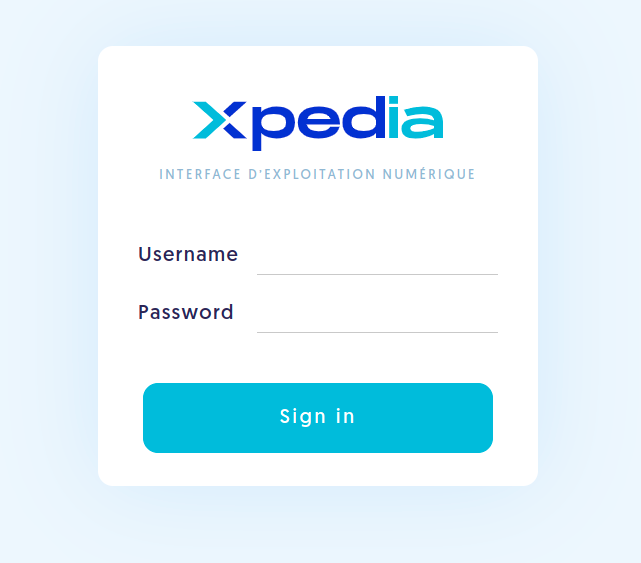
\includegraphics[width=0.8\textwidth]{xpedia_log.png}
    \caption{La login de Xpedia}\label{fig:xpedia_log}
\end{figure}
\begin{figure}[H]
    \centering
    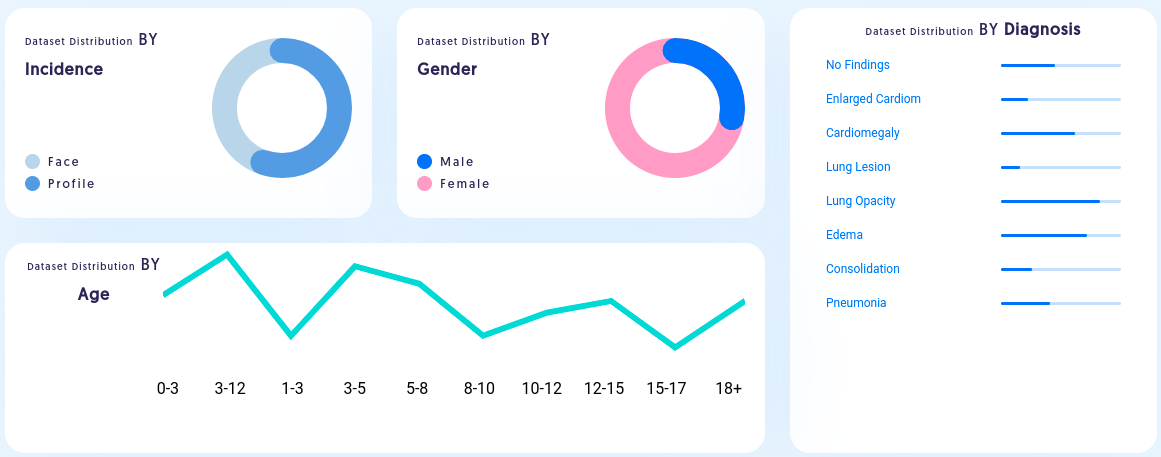
\includegraphics[width=0.8\textwidth]{xpedia_dashboard.png}
    \caption{Le dashboard}\label{fig:xpedia_dashboard}
\end{figure}
\begin{figure}[H]
    \centering
    
\includegraphics[width=0.8\textwidth]{xpedia_menu.png}
    \caption{La menu}\label{fig:xpedia_menu}
\end{figure}
\begin{figure}[H]
    \centering
    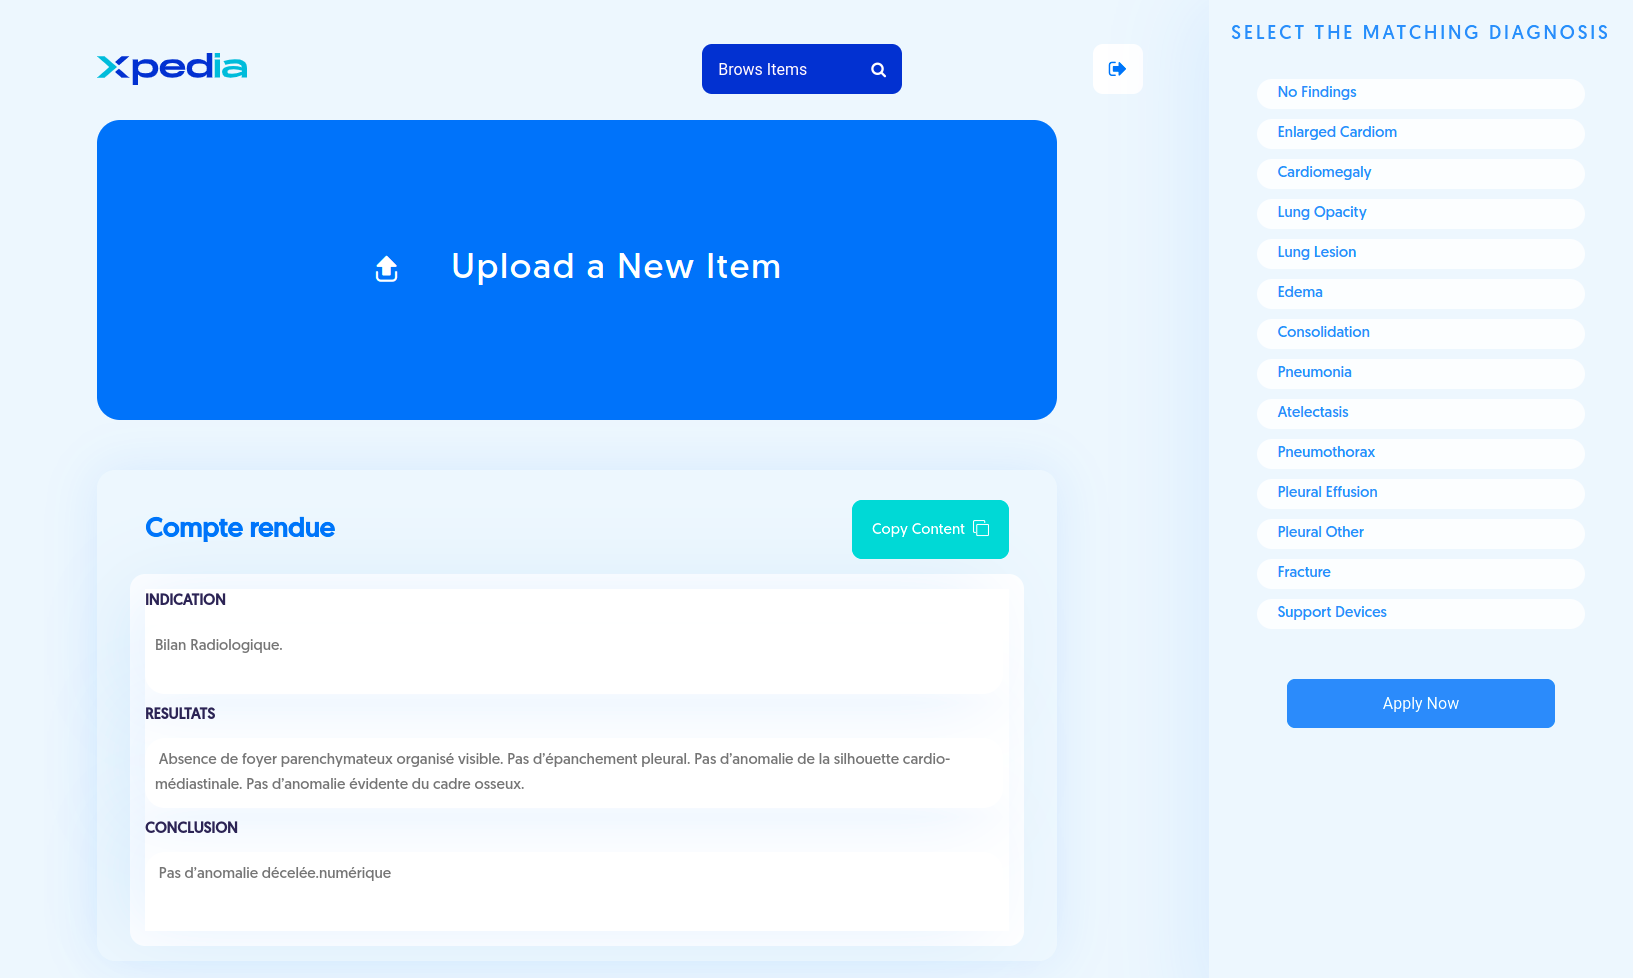
\includegraphics[width=0.8\textwidth]{xpedia_additem.png}
    \caption{La page ajouter élément}\label{fig:xpedia_additem}
\end{figure}
\begin{figure}[H]
    \centering
    
\includegraphics[width=0.8\textwidth]{xpedia_add_image.png}
    \caption{La section réserver à l'ajout d'une image}\label{fig:xpedia_add_image}
\end{figure}
\begin{figure}[H]
    \centering
    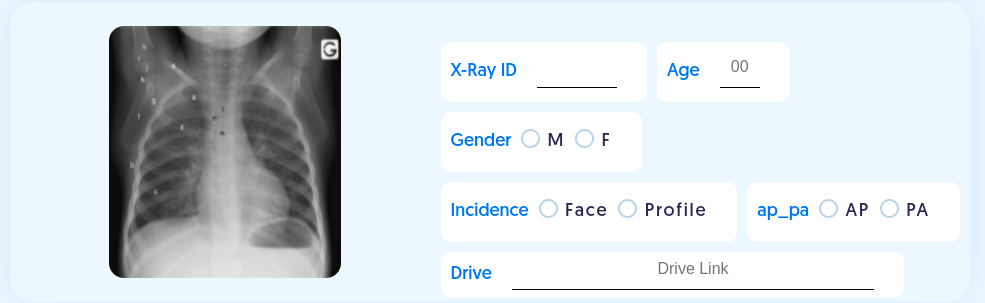
\includegraphics[width=0.8\textwidth]{xpedia_fill_form.png}
    \caption{La formulaire à remplir}\label{fig:xpedia_fill_form}
\end{figure}
\begin{figure}[H]
    \centering
    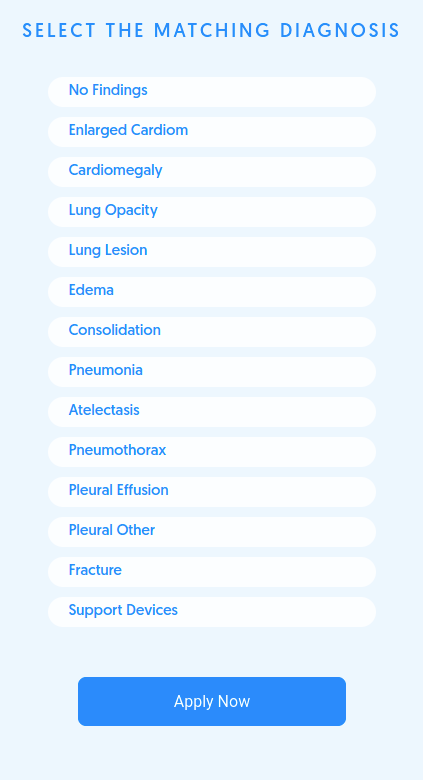
\includegraphics[width=0.8\textwidth]{xpedia_select_section.png}
    \caption{La section de selection des diagnostiques}\label{fig:xpedia_select_section}
\end{figure}
\begin{figure}[H]
    \centering
    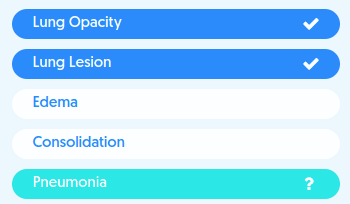
\includegraphics[width=0.8\textwidth]{xpedia_select_items.png}
    \caption{Exemple de selection des diagnostiques}\label{fig:xpedia_select_items}
\end{figure}
\begin{figure}[H]
    \centering
    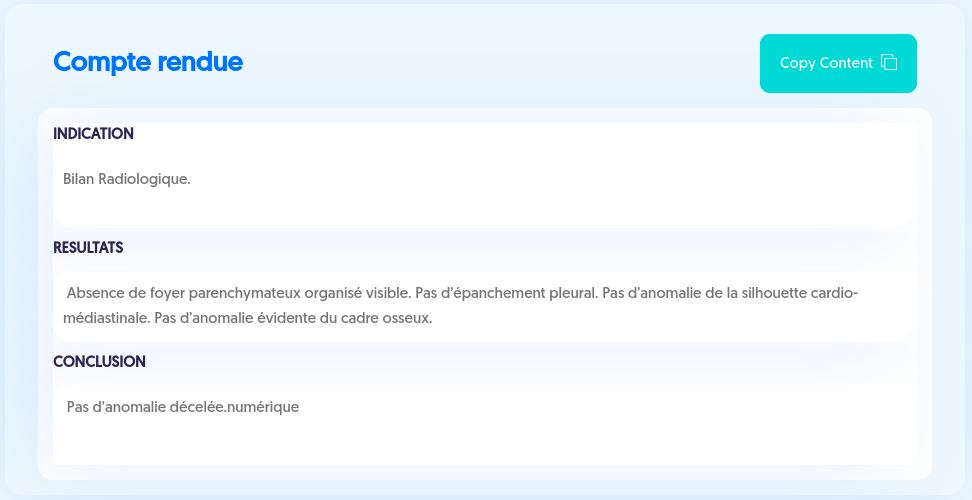
\includegraphics[width=0.8\textwidth]{xpedia_cr}
    \caption{La section du remplissage du compte rendue}\label{fig:xpedia_cr}
\end{figure}
\begin{figure}[H]
    \centering
    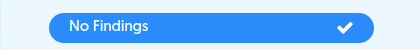
\includegraphics[width=0.8\textwidth]{xpedia_normal_select.png}
    \caption{Choix de 'No Finding' diagnostique}\label{fig:xpedia_menu}
\end{figure}
\begin{figure}[H]
    \centering
    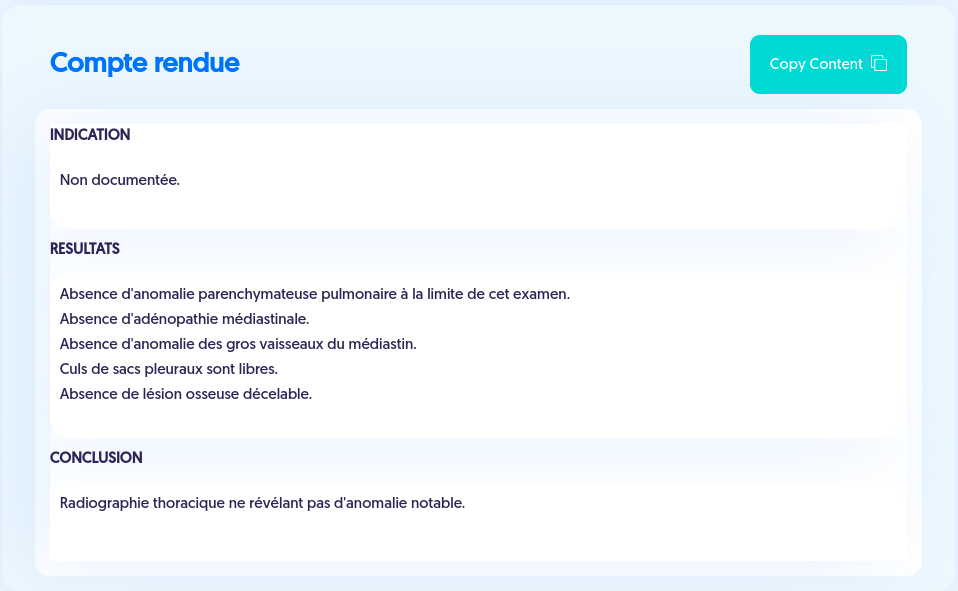
\includegraphics[width=0.8\textwidth]{xpedia_normal_cr.png}
    \caption{Remplissage automatique du compte rendue}\label{fig:xpedia_normal_cr}
\end{figure}
\begin{figure}[H]
    \centering
    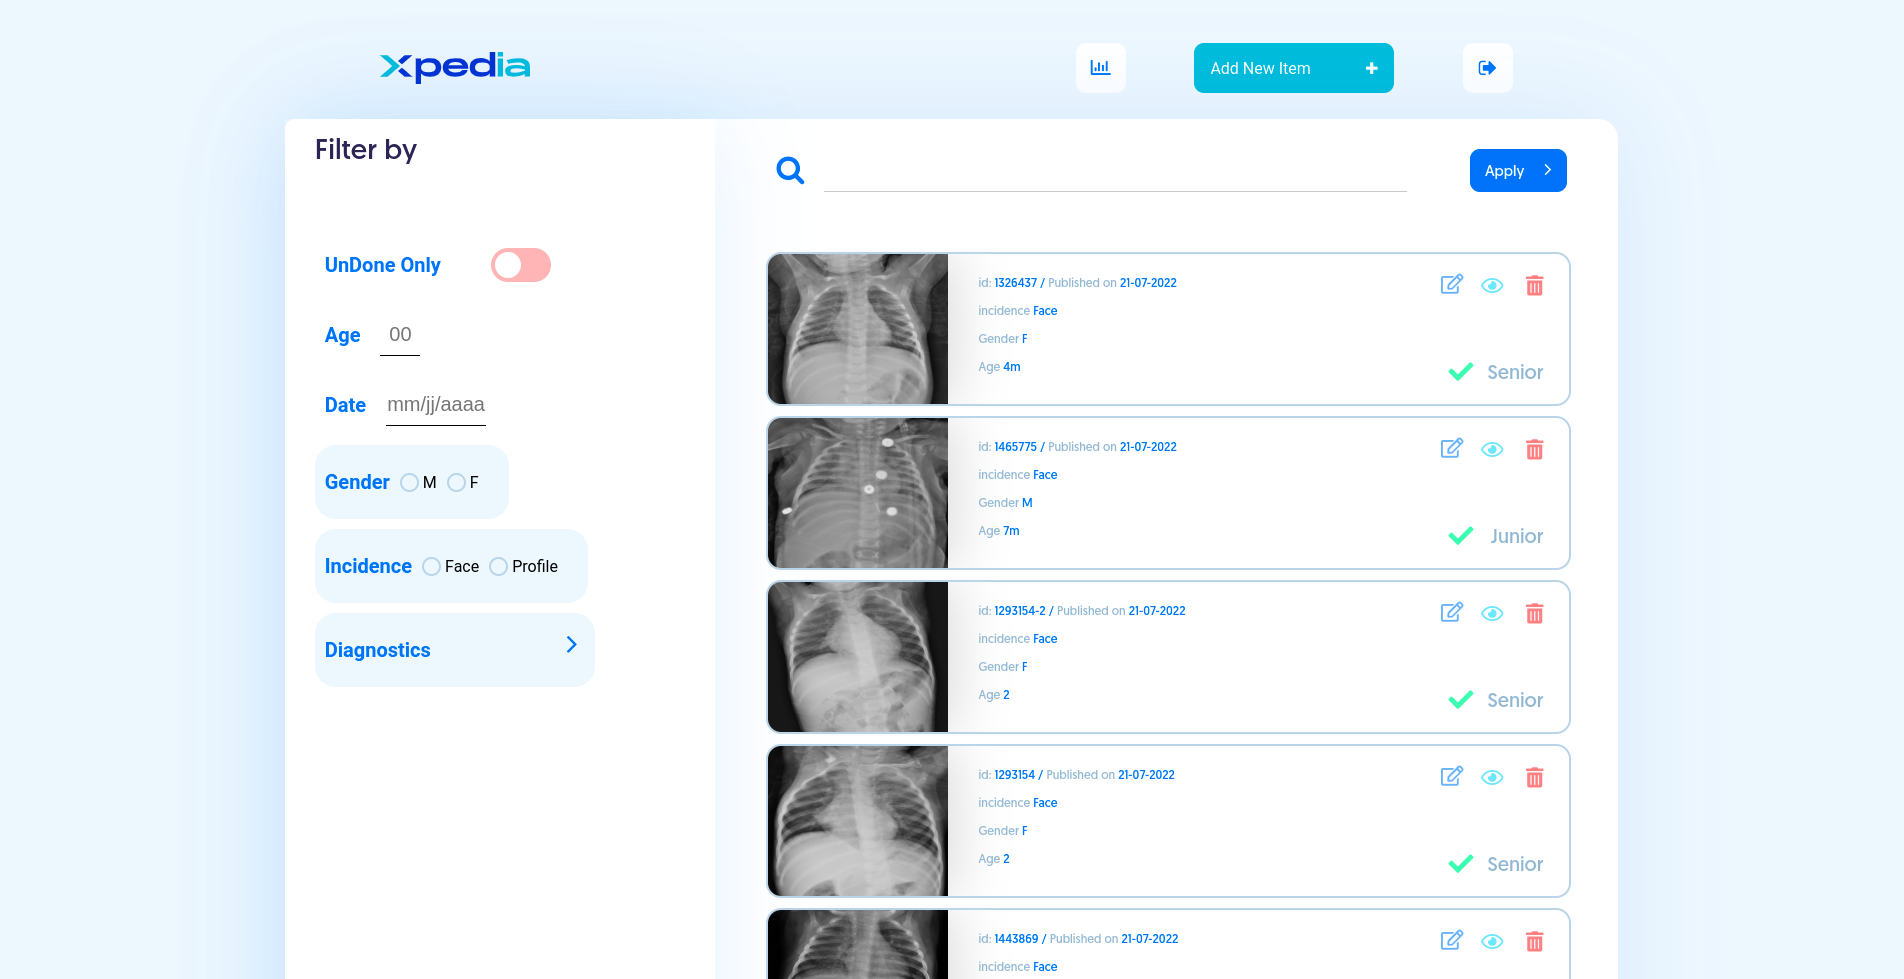
\includegraphics[width=0.8\textwidth]{xpedia_browse_item.png}
    \caption{La page 'browse items'}\label{fig:xpedia_menu}
\end{figure}
\begin{figure}[H]
    \centering
    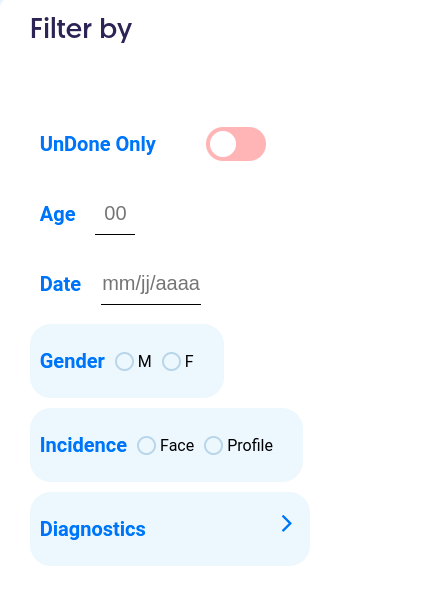
\includegraphics[width=0.8\textwidth]{xpedia_filter_section.png}
    \caption{La section du filtre des éléments}\label{fig:xpedia_filter_section}
\end{figure}
\begin{figure}[H]
    \centering
    
\includegraphics[width=0.8\textwidth]{xpedia_research.png}
    \caption{La bar de recherche}\label{fig:xpedia_research}
\end{figure}
\begin{figure}[H]
    \centering
    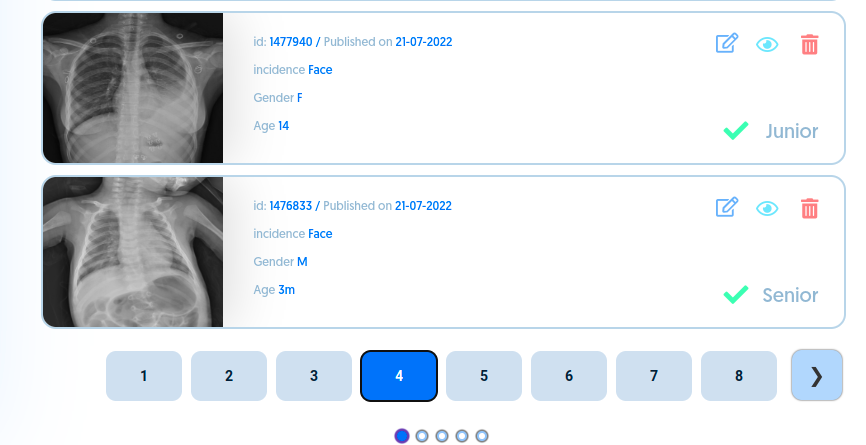
\includegraphics[width=0.8\textwidth]{xpedia_pagination.png}
    \caption{La menu}\label{fig:xpedia_menu}
\end{figure}
\begin{figure}[H]
    \centering
    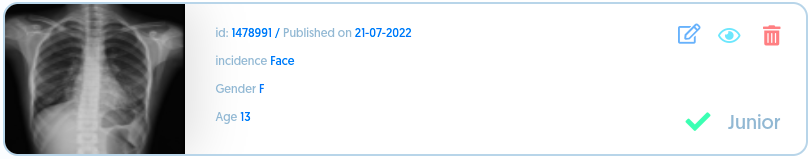
\includegraphics[width=0.8\textwidth]{xpedia_item_thumbnail.png}
    \caption{Vignette de l'élément}\label{fig:xpedia_item_thumbnail}
\end{figure}
\begin{figure}[H]
    \centering
    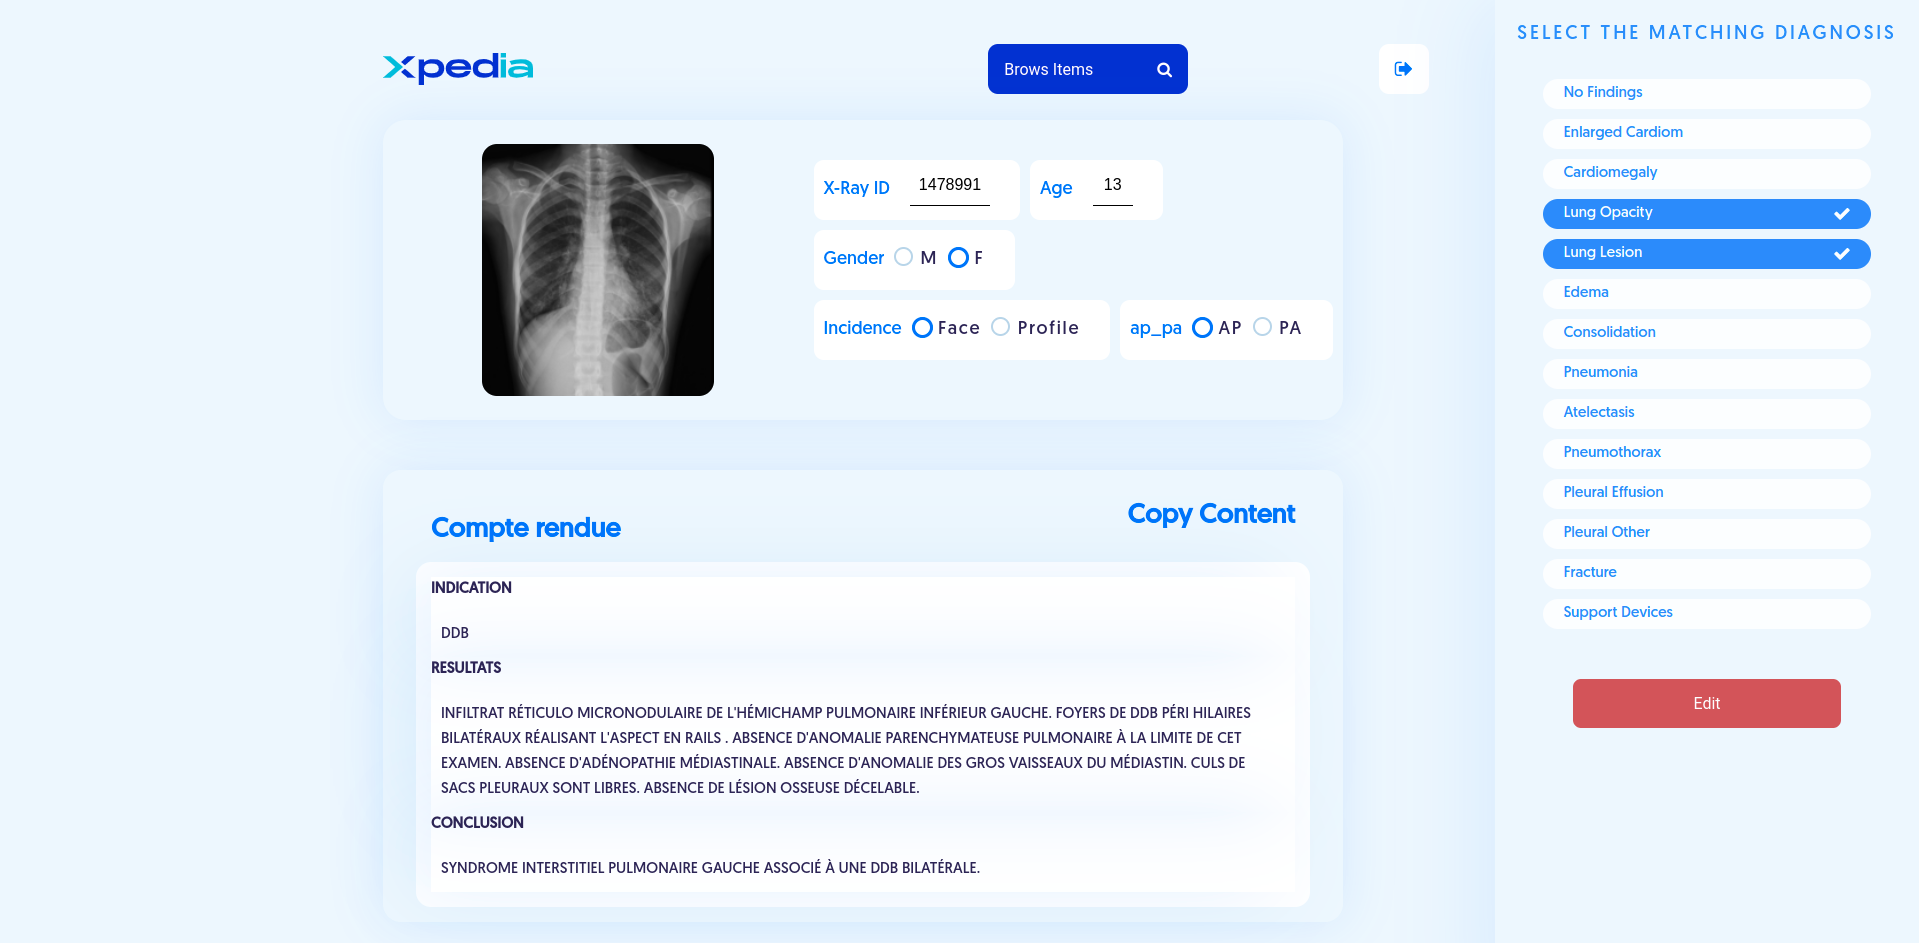
\includegraphics[width=0.8\textwidth]{xpedia_view_page.png}
    \caption{Les détailles de l'élément}\label{fig:xpedia_view_page}
\end{figure}
\begin{figure}[H]
    \centering
    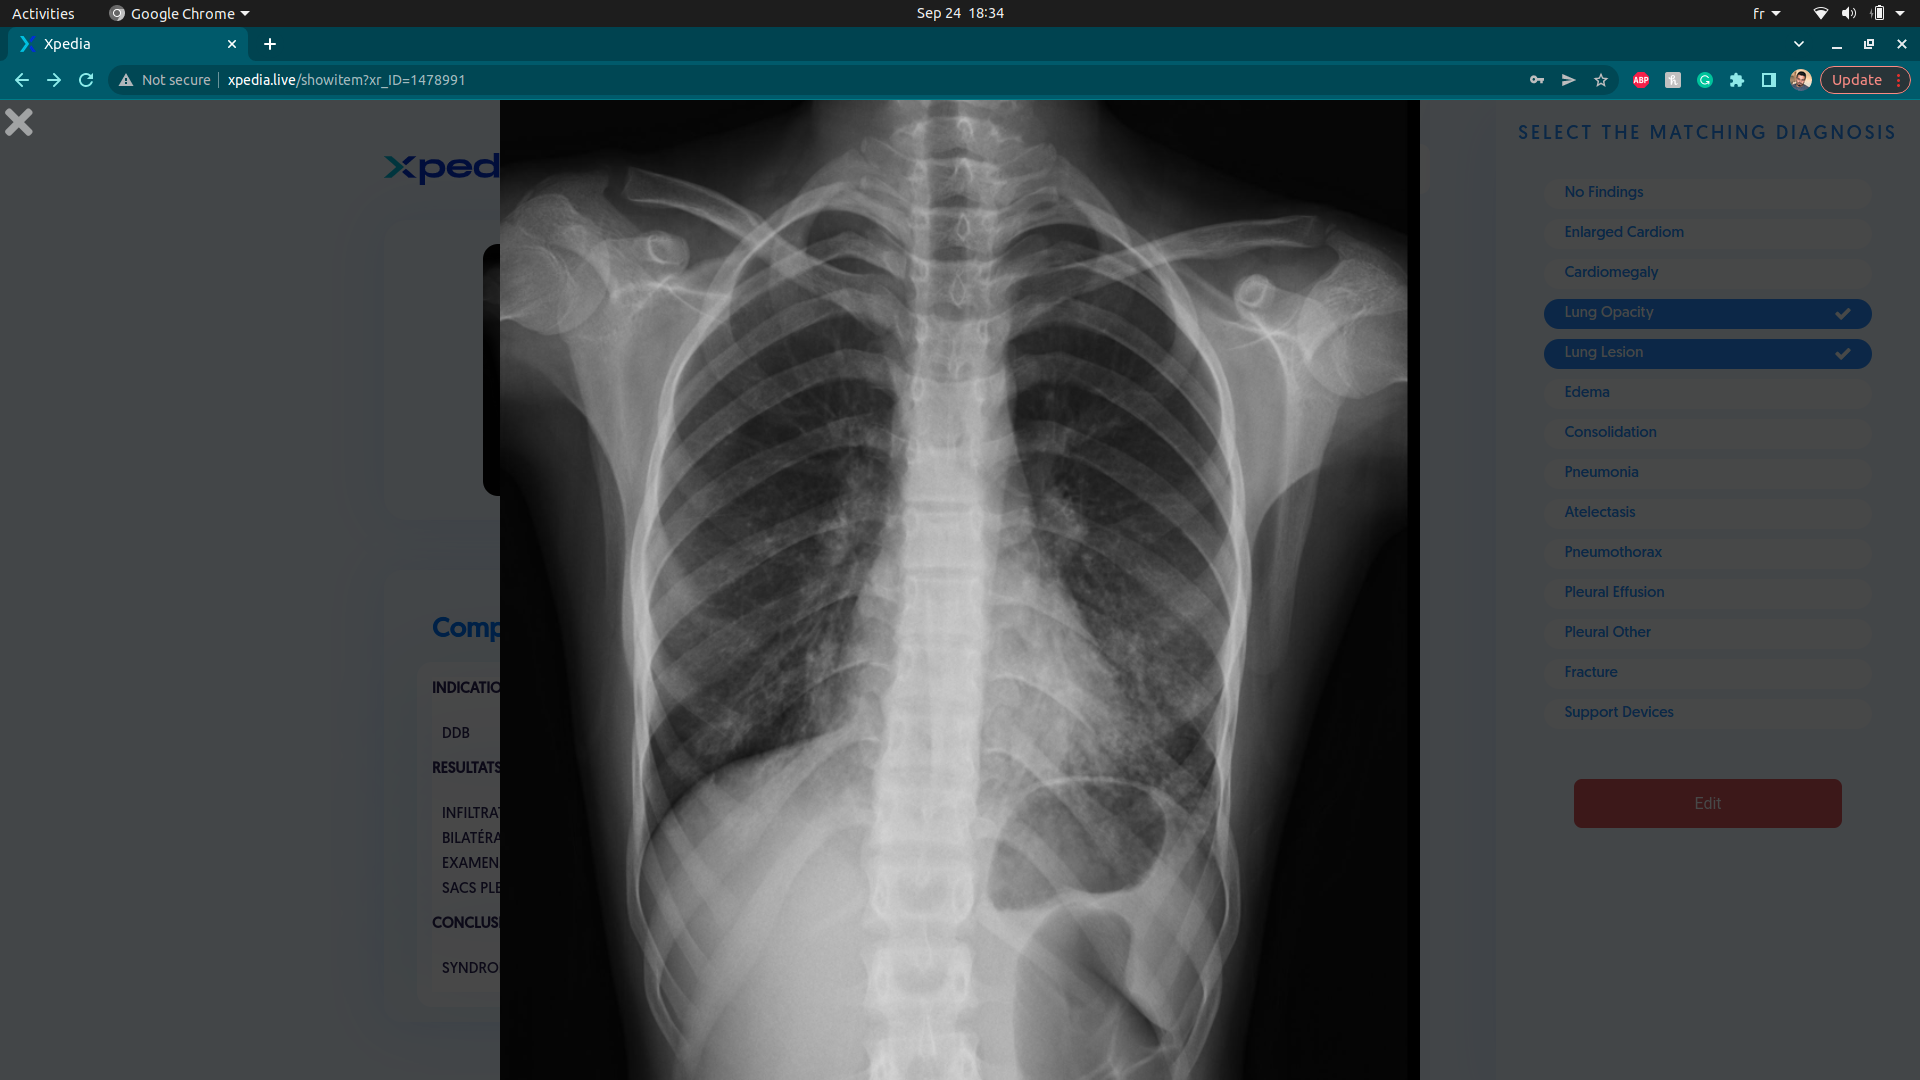
\includegraphics[width=0.8\textwidth]{xpedia_view_showitem.png}
    \caption{Clichés en dimension réel}\label{fig:xpedia_view_showitem}
\end{figure}
\begin{figure}[H]
    \centering
    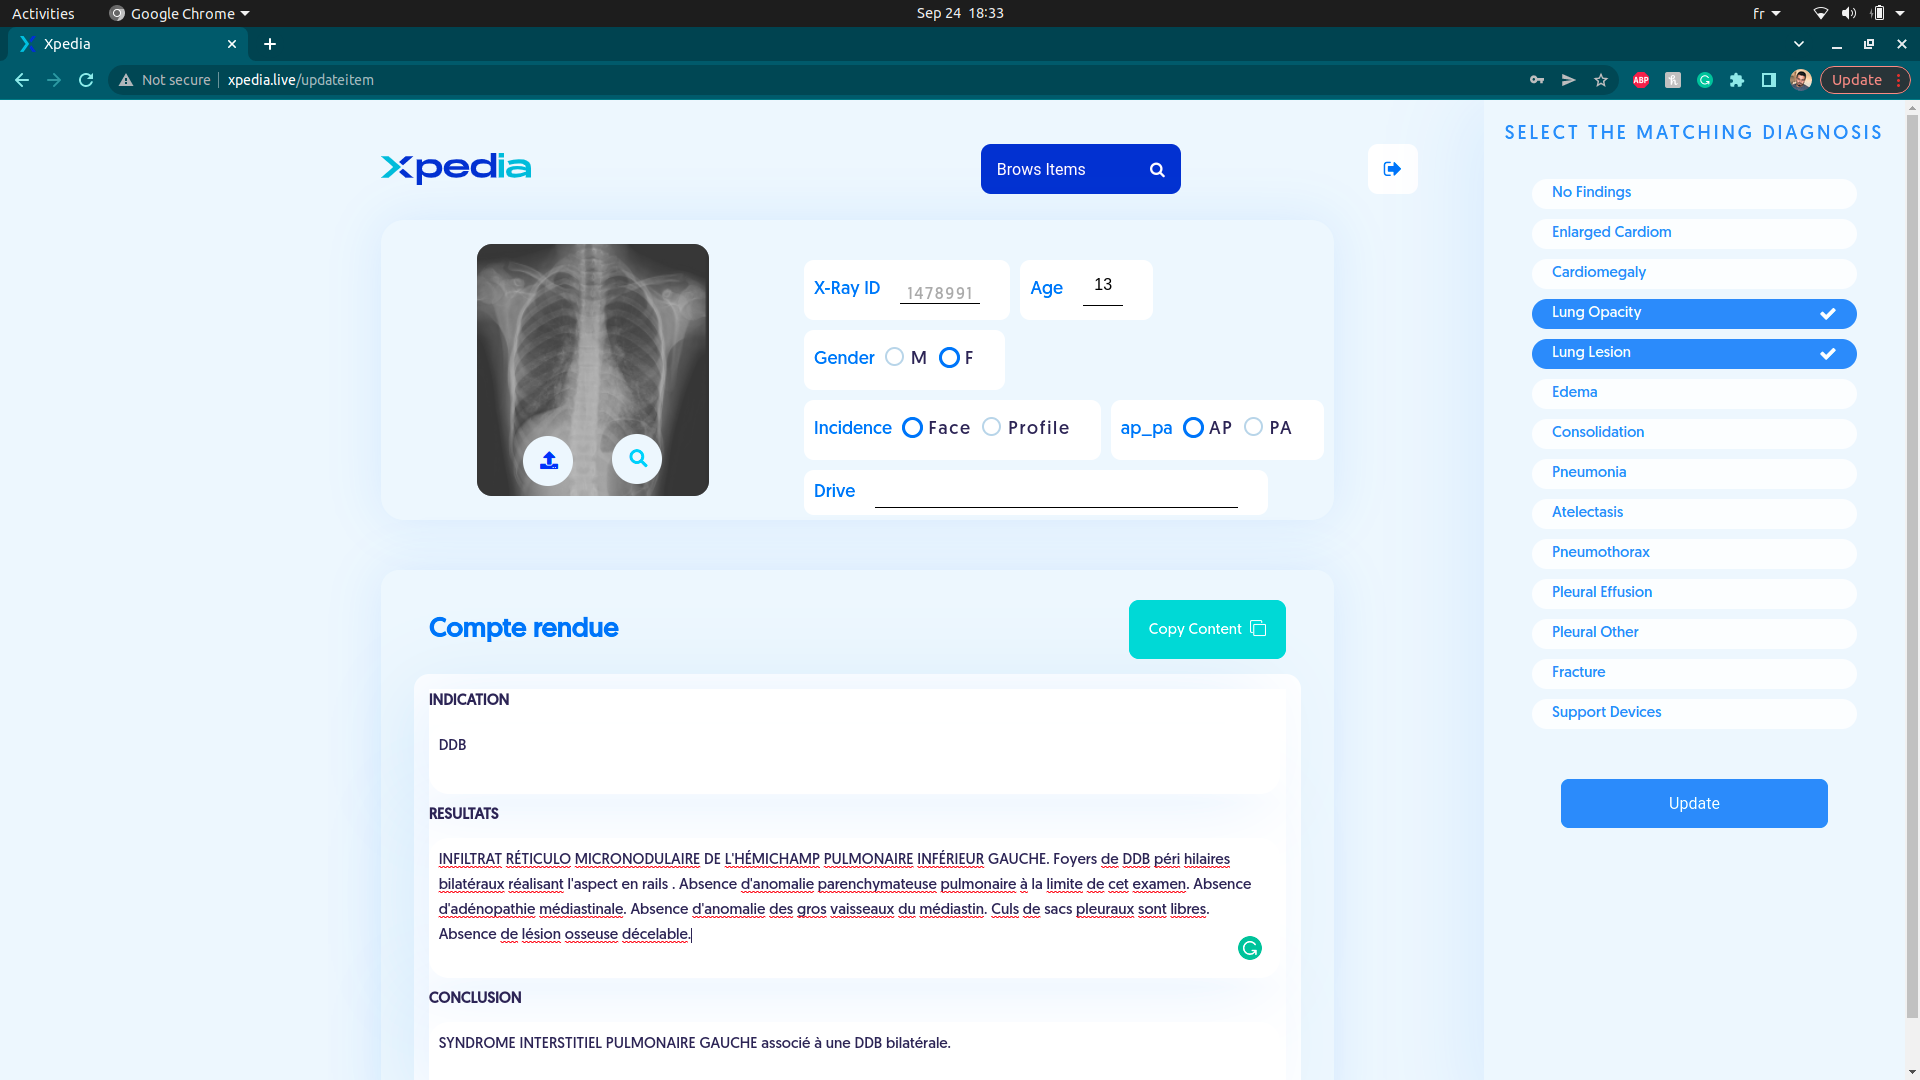
\includegraphics[width=0.8\textwidth]{xpedia_edit_page.png}
    \caption{La page d'edition de l'élément}\label{fig:xpedia_item_thumbnail}
\end{figure}
\subsection{Preparation des données}
La phase de préparation de données est l'une des phases cruciales dans le projet, le livrable de cette phase est le jeu de données qui alimente le modèle d'apprentissage en profondeur. Pour que ces données soient utiles, elles doivent d'abord être prétraitées selon les étapes déjà décrites dans la section \ref{data_pipeline}. Les figures présentent un exemple de traitement préparatif des données pour l'entraînement, le rest se trouve dans \ref{}.
\begin{figure}[H]
    \centering
    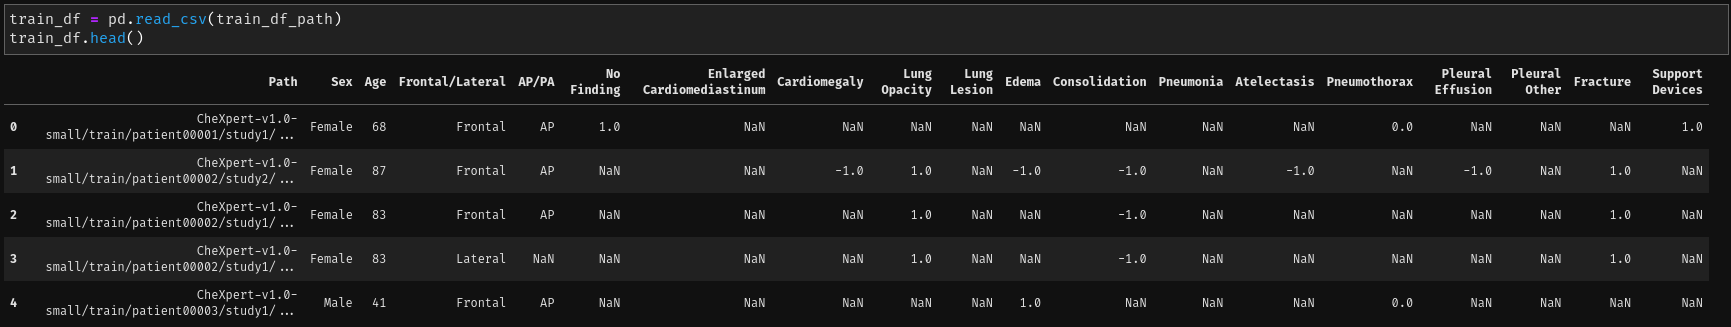
\includegraphics[width=0.8\textwidth]{raw_data.png}
    \caption{Les données brute de la base de données CheXpert}\label{fig:raw_data}
\end{figure}
\begin{figure}[H]
    \centering
    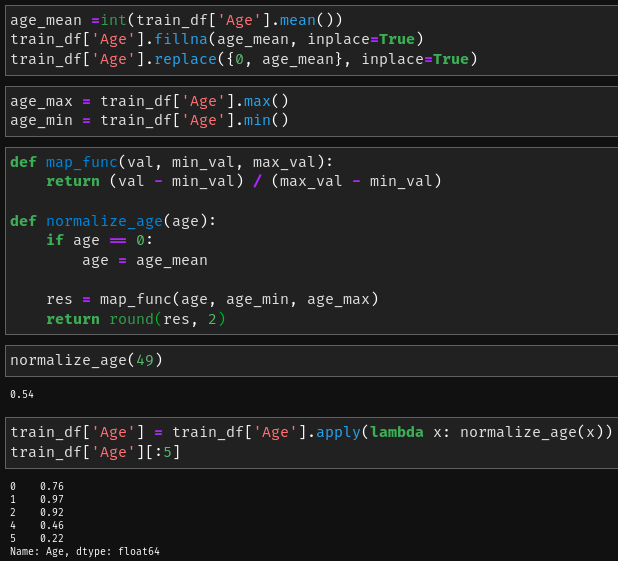
\includegraphics[width=0.8\textwidth]{age_prep.png}
    \caption{La préparation de la colone 'Age'}\label{fig:age_prep}
\end{figure}
\begin{figure}[H]
    \centering
    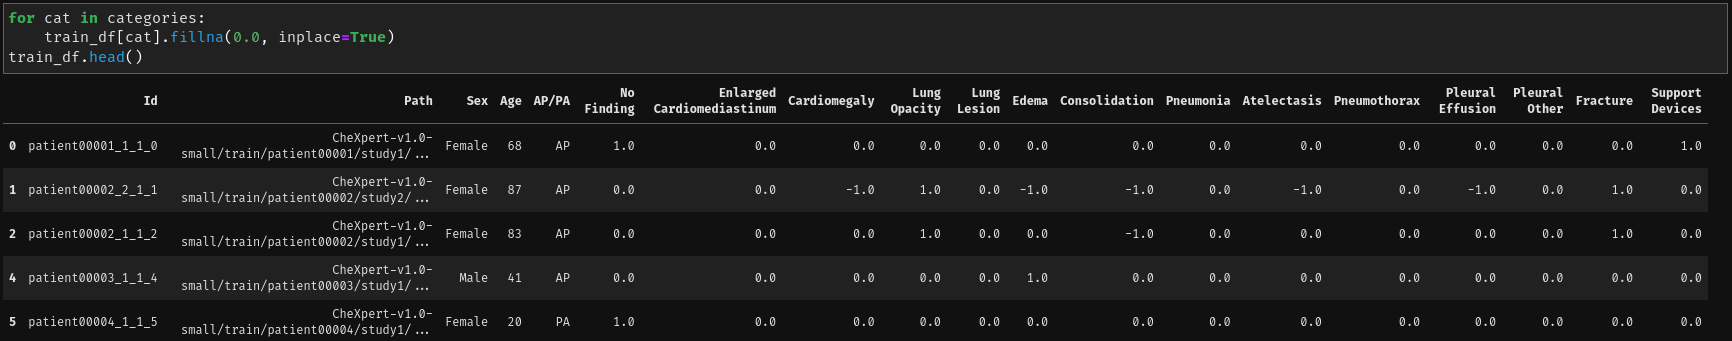
\includegraphics[width=0.8\textwidth]{nan_fill.png}
    \caption{Remplacer les celles vides (Nan)}\label{fig:nan_fill}
\end{figure}

On constate que notre jeu de données comporte plus de 200000 images qui doivent être redimensionnées et convertis en un tableau numpy pour les utiliser comme des entrées dans la phase d'entraînement, cela génère un goulot d’étranglement de flux d’opération. Alors pour anticiper cela on va faire les opérations de prétraitement d’image une seule fois à l'avance et enregistrer le rendu sous forme de fichiers. Et par la suite utiliser ces derniers dans la phase d'entraînement.

\begin{figure}[H]
    \centering
    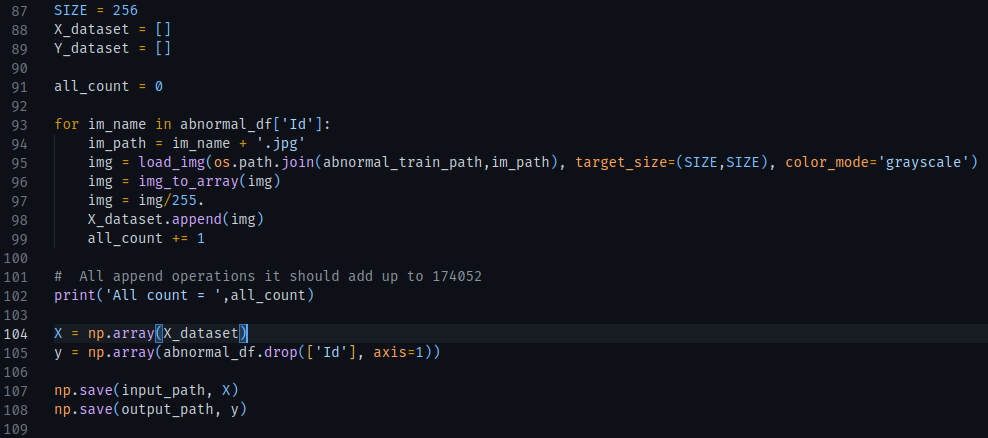
\includegraphics[width=0.8\textwidth]{input_output.png}
    \caption{Préparer les images et meta données pour la phase d'entraînement}\label{fig:input_output}
\end{figure}


\subsection{Madèles d'apprentissage en profondeur}
Dans cette phase, nous avons essentiellement deux voies principales à suivre, comme indiqué sur la figure, la première consiste à créer notre propre modèle et à commencer à l'entraîner sur les données préparées, et la deuxiéme consiste à utiliser un modèle pré-entraîner pour se recycler sur le données préparées, mais quel que soit la voie que nous choisissons, la structure de notre modèle sera la même.
Notre structure n'est pas simple car nous avons deux types de données d'entrée, nous avons donc deux modèles distincts pour traiter chaque type, puis les concaténer dans une couche entièrement connectée pour accéder à notre couche de sortie.
Dans les paragraphes suivants, nous parlerons des couches et de modèles Keras.
D’abord en commençant par le modèle binaire pour classer les données normales et anormales, pour le modèle de traitement d'images nous allons construire un modèle séquentiel contenant:
\begin{enumerate}
    \item couche Conv2D avec la fonction d'activation Relu
    \item couche de BatchNormalization
    \item Couche de Maxpooling
    \item Couche de Dropout (pas toujours)
\end{enumerate}
En répétant ces 4 couches 3 à 4 fois en réglant les paramétres relatives à chaque couche (nombre de filtres, taille de pooling, valeur de dropout …) on va avoir la partie de base de notre modèle, aprés on va finalisé notre modèle par les couches suivantes:
\begin{enumerate}
    \item couche Flatten
    \item couche Dense avec la fonction d'activation Relu
    \item couche Dropout
    \item couche Dense avec la fonction d'activation Relu
    \item couche Dropout
    \item couche Dense avec la fonction d'activation Sigmoid
\end{enumerate}

Puis pour le modèle de traitement du meta données (Age, Sexe, AP/PA), on va utiliser un modèle séquentiel contenant 2 couches Dense avec la fonction d’activation Relu.

Et finalement on doit combiner ces 2 modèle par 2 couches Dense avec fonction d’activation Relu pour avoir la couche de sortie de notre modèle principale.

La sortie de ce modèle et un nombre compris entre 0 et 1.

Pour le modèle multi-etiquettes on aura la même structure avec la différence du format de la sortie qui sera un tableau de valeurs entre 0 et 1, ce dernier représente la probabilité d'existence de chaque pathologie respectivement.


\section{Experiences}

Dans cette partie on aura une vision totale sur les expériences effectuées et les expériences en attente de réalisation en raison du problème de ressources déjà expliqué dans la partie précédente.

Comme on le voit sur la figure, l'historique des expériences faites pour créer un modèle binaire montre qu’après un changement de la taille des images nous avons gardé la même structure tout en incrémentant le nombre d'époques, car il a eu une évolution évidente de la précision du modèle.


Pour le modèle multi-étiquettes on a déjà réalisé 6 expériences avec des changements dans les paramètres surtout:
\begin{enumerate}
    \item La taille des filtres pour qu’ils mieux couvre la totalités de l’image sans avoir un débordement
    \item Réduire la taille de Pooling pour ne pas avoir une chute dans la taille du rendu de cette couche
    \item Augmenter la taille des images et finalement varier les valeur de la couche Dropout pour augmenter la valeur du rappel du modèle
    \item Augmenter taille du lot pour avoir un taux d'apprentissage plus grand
\end{enumerate}
on n'a pas pu effectuer l'entraînement de toutes les structures créées mais voici quelques exemples d'expériences futures:
\begin{enumerate}
    \item Prends les modèles résultant des expériences précédentes et les alimenter par le jeu de données de la population pédiatrique pour avoir des modèles de classification binaire/multi-etiquettes réservé à la population pédiatrique.
    \item Alimenter un modèle pre-entraîné par les données de la population adulte pour avoir un modèle binaire de classification (normal/anormal).
    \item Alimenter un modèle pre-entraîné par les données de la population adulte pour avoir un modèle de classification multi-etiquettes pour classifier le reste des anomalies.
    \item Réduire le nombre de sortie, en choisissant les anomalies avec la plus grande présence dans la base de données.
    \item Un modèle binaire pour chacune des anomalies, combinées dans un modèle globale par 2 couches Dense une avec La fonction d'activation Relu et la dernière avec la fonction d'activation Sigmoid.
    \item Appliquer l'expérience 1. sur les modèles résultant des expériences 2., 3., 4., 5.
\end{enumerate}

chacune des expériences précédentes aura un certain nombre d'expériences enfants lors du changement des paramètres ou des tailles utilisés.



\section{Résultats}

\section*{Conclusion}